%% AAAI-27 anonymous submission working source.
\documentclass[letterpaper]{article}
\usepackage[submission]{aaai2027}
\usepackage[hyphens]{url}
\usepackage{graphicx}
\urlstyle{rm}
\def\UrlFont{\rm}
\usepackage{natbib}
\usepackage{caption}
\frenchspacing

\usepackage{booktabs}
\usepackage{multirow}
\usepackage{amsmath}
\usepackage{amssymb}
\usepackage{xcolor}

\pdfinfo{
/TemplateVersion (2027.1)
}

\setcounter{secnumdepth}{1}
\graphicspath{{figures/}}

\title{Anomaly-Targeted Retrieval: Selective Re-Reading for Training-Free Long-Video Anomaly Understanding}
\author{Anonymous Submission}
\affiliations{}

\begin{document}

\maketitle

\begin{abstract}
Long-video anomaly understanding requires broad scene context and sensitivity to brief, sparse event evidence, yet a single uniformly sampled view can underemphasize the moments that determine the final decision.
We introduce \textit{A}nomaly-\textit{T}argeted \textit{R}etrieval (\textit{ATR}), a training-free selective re-reading framework.
Scout first searches the complete video for candidate evidence; Sniper then jointly receives the same complete video and the retrieved clip, preserving global context while adding a denser second view without parameter updates or target-task temporal supervision.
On the official UCF-Crime test set, ATR raises a 4B model to 85.17\% accuracy and reduces its false-negative rate from 26.43\% to 11.43\%.
An 8B configuration reaches 85.52\% accuracy with 9.33\% false-positive rate, outperforming a 32B global-only baseline at about one tenth of its GPU-hour cost.
Compute- and content-matched controls show that a second global call alone provides no gain, while Scout significantly outperforms duration-matched Random and Uniform clips in the 4B setting.
Removing the retrieved view reverses all analyzed rescued decisions, confirming that the final prediction uses the selected evidence.
Together, these results establish content-aware global--local retrieval as a practical and efficient inference strategy for long-video anomaly understanding.
\end{abstract}
    


%% ============================================================
%% MAIN CONTENT
%% ============================================================

\section{Introduction}

% In real-world surveillance and content moderation, anomalous events exhibit a
% ``needle-in-a-haystack'' property---criminal actions may span only seconds within long
% surveillance footage. With the emergence of Vision-Language Models (VLMs) built upon powerful foundations like CLIP~\cite{radford2021learning} and SigLIP~\cite{zhai2023sigmoid}, the field is shifting
% from shallow ``anomaly detection'' (VAD) toward deeper ``anomaly understanding''
% (VAU)~\cite{zhang2024holmes,pi2024vader}, demanding precise event localization, low false
% negative rates, and semantic explanations.

% Despite demonstrating strong zero-shot capabilities on short clips, standard VLMs encounter three critical bottlenecks when deployed on long-form surveillance footage: (1)~\textbf{``Weak Cause--Strong Effect'' misalignment}---the actual
% criminal action (concealed weapon drawing, the ``weak cause'') occupies only seconds, while
% crowd panic (the ``strong effect'') dominates visual change; attention-driven VLMs are drawn
% to the effect, missing the causal onset. (2)~\textbf{Single-pass attention forgetting}---full
% video inference incurs $O(L^2)$ complexity~\cite{vaswani2017attention}, causing subtle early
% events to be overwhelmed by background tokens. (3)~\textbf{Text-mediated information loss}---
% pipelines that convert video to captions (e.g., LAVAD~\cite{zanella2024harnessing}) lose the
% pixel-level micro-evidence needed to detect concealed anomalies.

% To dismantle these barriers, we propose \textbf{Anomaly-Targeted Retrieval (ATR)}, a training-free Visual RAG framework
% that introduces \textbf{Hierarchical Visual Repetition} to the video domain. Inspired by
% RAG~\cite{lewis2020retrieval}, ATR performs \emph{intra-video retrieval} via a
% \emph{VLM-as-a-Retriever} mechanism, achieving temporal grounding while eliminating the need for temporal annotations or parameter fine-tuning. ATR employs a coarse-to-fine dual-stage architecture: \textbf{Scout} globally
% scans for candidate anomalous windows; \textbf{ACE} (Asymmetric Causal Expansion) pads
% windows with aggressive look-back to capture action onset; \textbf{Sniper} jointly processes
% the full global video and the ACE-trimmed focused clip, achieving \textbf{Temporal Zoom-in}
% via heterogeneous dual-view reasoning.

% Video anomaly understanding aims not only to determine whether a long video contains abnormal events but also to identify when they occur and why they should be considered anomalous. 
% Video anomaly understanding aims to determine whether a long video contains abnormal events, provide coarse evidence about where they occur, and explain why they may be considered anomalous. This capability is important for multimedia applications such as surveillance analysis~\cite{sultani2018real}, public safety monitoring, and content moderation. Recent vision-language models (VLMs)~\cite{radford2021learning,zhai2023sigmoid} have shown strong zero-shot performance on short video understanding tasks, suggesting a promising direction toward training-free anomaly understanding. However, their effectiveness remains limited in long-form videos, where abnormal events are often sparse, subtle, and embedded in a lengthy normal context.

Video anomaly understanding aims to determine whether a long video contains abnormal events, retrieve evidence about where they may occur, and explain why they may be considered anomalous. This capability is important for a broad range of multimedia applications, including surveillance analysis, public safety monitoring, and content moderation~\cite{sultani2018real}. Recent vision-language models (VLMs)~\cite{radford2021learning,zhai2023sigmoid} have shown promising zero-shot performance on short video understanding tasks, suggesting a potential path toward training-free anomaly understanding. However, extending this ability to long-form videos remains difficult, since anomalous events are often sparse, subtle, and embedded in lengthy normal context. In this work, candidate timestamps are an intermediate retrieval interface; the final task is video-level judgment and semantic reasoning, not calibrated frame-level boundary prediction.


A central difficulty is selective access to temporal evidence. In surveillance footage, the decisive action may occupy only a few seconds, while the complete scene is still needed to determine whether that action is anomalous. Uniform full-video inference can underemphasize sparse evidence, whereas local-only inference removes the context required for verification. Existing approaches therefore face a tension between \textit{local sensitivity} and \textit{global contextual understanding}. This challenge is further aggravated by the cost of long-context attention~\cite{vaswani2017attention} and by caption-mediated pipelines~\cite{zanella2024harnessing} that may discard subtle visual cues.

% To address these issues, we propose \textbf{A}nomaly-\textbf{T}argeted \textbf{R}etrieval (\textbf{ATR}), a training-free framework for long-form video anomaly understanding. ATR performs coarse-to-fine temporal grounding within a video: it first scans the full video to identify candidate anomalous intervals, then expands the detected interval asymmetrically to recover likely causal context, and finally jointly reasons over the original video and a focused temporal clip. This dual-view design increases the proportion of anomaly-relevant evidence available to the model while preserving global scene context, enabling more reliable anomaly-centric reasoning without temporal annotations or parameter updates.

To address these issues, we formulate anomaly understanding as content-relevant intra-video retrieval followed by global--local verification. Based on this formulation, we propose \textbf{A}nomaly-\textbf{T}argeted \textbf{R}etrieval (\textbf{ATR}), a training-free two-call framework. Scout first scans the complete video and proposes candidate intervals. Sniper then receives two visual inputs together: the same complete original video and a focused clip cut from it. The complete video is never replaced by a crop; the local clip provides a denser second view while the full video preserves scene and temporal context. A fixed temporal padding rule supplies surrounding context before clip extraction. The framework requires neither temporal annotations nor parameter updates.

\begin{figure*}[t]
  \centering
  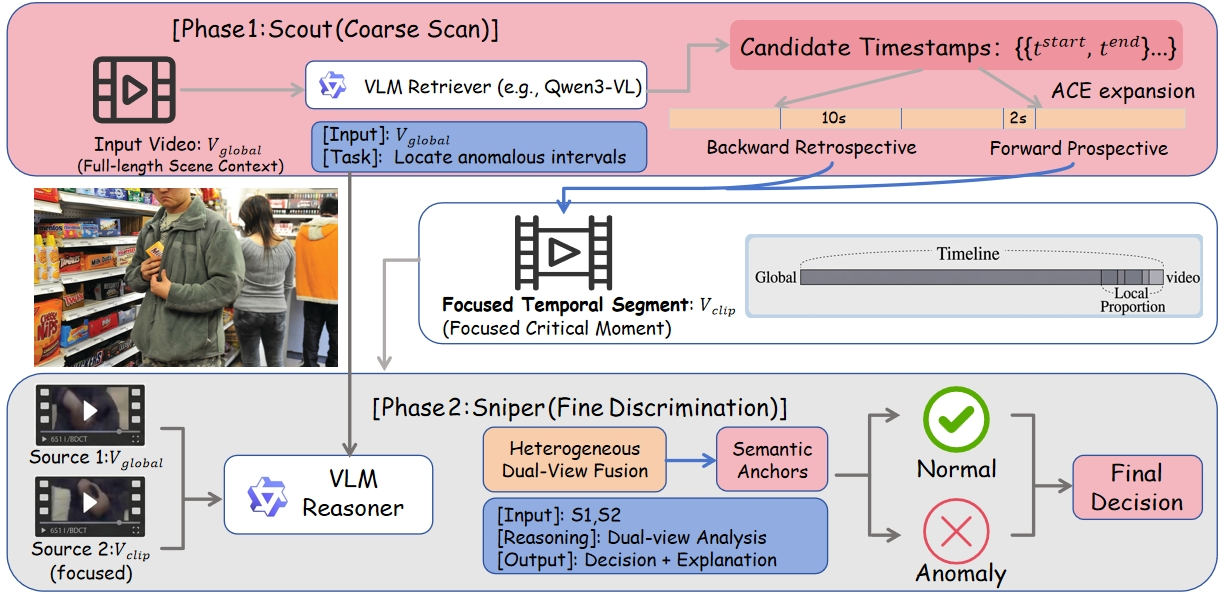
\includegraphics[width=0.915\linewidth]{figures/fig_framework.png}
  \caption{Overview of the ATR framework. The Scout module performs global scanning to
  identify candidate anomalous windows. A fixed temporal padding rule retains nearby context before clip extraction. The Sniper
  module performs heterogeneous dual-view reasoning over the full global video and the
  focused temporal segment simultaneously.}
  \label{fig:framework}
\end{figure*}
Extensive experiments on UCF-Crime show that ATR substantially reduces missed anomalies for lightweight VLMs. Strict matched controls separate content selection from an extra model call, additional tokens, and arbitrary clips, while evidence-removal tests verify that Sniper uses the retrieved view. An 8B ATR configuration also outperforms a substantially larger 32B global-only baseline at about one tenth of its GPU-hour cost. Additional experiments across model families and an audio-visual benchmark characterize how the operating point transfers beyond the primary setting.

The main contributions can be summarized as follows:

% \begin{enumerate}
%   % \item \textbf{Hierarchical Visual Repetition and the ATR Framework}: We introduce \textbf{Hierarchical Visual Repetition}, enabling efficient heterogeneous dual-view reasoning. With only $\sim$5\% additional tokens, ATR reduces the 4B model's FNR by 56.8\% relative to baseline and achieves 85.17\% accuracy. The 8B model reaches 85.52\%, surpassing the 32B baseline (83.45\%), proving that intelligent retrieval can substitute for model scale.

%   % \item \textbf{ACE: Asymmetric Causal Expansion}: A targeted temporal calibration mechanism addressing ``weak cause--strong effect'' asymmetry. Validated as a reliable positive calibrator, ACE consistently improves FNR and F1 without degrading accuracy, scaling with Scout localization precision.

%   % \item \textbf{Over-Alignment Phenomenon}: We identify that excessive safety alignment in 32B models compromises sensitivity. ATR yields negative gains on 32B but positive gains on 4B/8B, attributed to 32B's high Scout failure rate (62.4\%) and safety alignment interference~\cite{ouyang2022training,askell2021general}.

%   \item We propose ATR, a training-free framework that formulates long-form video anomaly understanding as an intra-video coarse-to-fine retrieval problem. ATR combines global scanning, asymmetric causal expansion to recover pre-anomaly context, and dual-view reasoning---enabling anomaly understanding without temporal annotations or parameter updates.

%   \item Through extensive experiments on UCF-Crime, XD-Violence, and multiple VLM backbones (Qwen3-VL, Qwen3.5-VL, Qwen2.5-Omni), we show that ATR consistently benefits lightweight models while revealing a dual-stage over-alignment phenomenon in larger models. These findings delineate empirical applicability boundaries for retrieval-augmented video understanding.
% \end{enumerate}

\begin{itemize}
    \item We propose \textbf{ATR}, a training-free selective re-reading framework that jointly presents the complete video and a content-relevant local view, preserving global context without temporal annotations or parameter updates.
    
    \item We provide a \textbf{mechanism-focused evaluation} using Second Global, duration-matched Random and Uniform clips, and Source~2 removal. These controls distinguish extra computation, token volume, content selection, and actual evidence use.
    
    \item We establish practical \textbf{accuracy--efficiency operating points}: ATR enables lightweight VLMs to reduce missed anomalies and outperform a 32B global-only baseline at roughly 10\% of its GPU-hour cost, with FNR/FPR and cross-backbone results reported jointly.
\end{itemize}


\section{Related Work}

\subsection{Video Anomaly Detection: From Signal Reconstruction to Semantic Understanding}

Traditional Video Anomaly Detection (VAD) has evolved through two dominant paradigms.
\textbf{Unsupervised methods} operate on the assumption that anomalies are deviations from learned normal patterns, using reconstruction or prediction errors as anomaly scores on benchmarks like ShanghaiTech~\cite{luo2017revisit}, Avenue~\cite{lu2013abnormal}, and UCSD Ped2~\cite{li2013anomaly}. Representative works include reconstruction-based and prediction-based approaches~\cite{gong2019memorizing,park2020learning,liu2018future}.
\textbf{Weakly-supervised methods} leverage video-level labels with Multiple Instance Learning (MIL)~\cite{sultani2018real,tian2021weakly,lv2023unbiased,zhang2024mtfl}, with recent extensions incorporating feature refinement~\cite{feng2021mist,wan2021weakly,wu2022self} and language supervision~\cite{wu2024vadclip,gu2024anomalygpt,wu2024open}.

These methods use task-specific supervision and usually optimize frame- or snippet-level ranking metrics. They are important localization baselines, but their supervision and output granularity differ from ATR's training-free video-level decision setting; we therefore discuss them as complementary rather than treating their reported frame-level scores as directly interchangeable with our metrics.

\subsection{Explainable and Training-Free Video Anomaly Understanding}

Recent VLM-based work extends VAD from anomaly scoring toward open-world description and explanation. HAWK~\cite{tang2024hawk} integrates motion-language supervision and trains on annotated anomaly descriptions and question--answer pairs. Holmes-VAU~\cite{zhang2024holmes} introduces multi-granular instruction data and an anomaly-focused temporal sampler for long-term understanding. VERA~\cite{ye2025vera} learns verbalized guiding questions from coarsely labeled data, while Follow the Rules (AnomalyRuler)~\cite{yang2024follow} induces scenario-specific rules from few-shot normal references before frame-level deduction. These methods are closely related in semantic scope, but use additional training data, learned components, or scenario references.

Training-free methods remove model updates but still differ in evidence construction and output. LAVAD~\cite{zanella2024harnessing} converts sampled visual content into text and obtains frame-level anomaly scores through language reasoning, while VADTree~\cite{li2025vadtree} organizes multi-granularity event nodes for explainable frame-level scoring. ATR instead retrieves candidate evidence directly from the input video and jointly presents that visual evidence with the complete video for a video-level decision. It does not claim to replace calibrated frame-level localization methods.

\begin{table*}[t]
  \centering
  \caption{Positioning against reviewer-identified related work. Reported scores are not mixed because supervision, task, and output granularity differ. ``Training-free'' here means no model-parameter update for the target task.}
  \label{tab:setting_comparison}
  \resizebox{\textwidth}{!}{%
  \begin{tabular}{lllll}
    \toprule
    Method & Target setting & Target-task supervision & Primary output & Relation to ATR \\
    \midrule
    VideoAgent~\cite{wang2024videoagent} & Long-video QA & None at evaluation; multiple tools & Answer & Agentic search, not VAD \\
    LITA~\cite{huang2024lita} & Temporal localization & Timestamped instruction tuning & Temporal span + text & Trained localizer \\
    VadCLIP~\cite{wu2024vadclip} & Weakly supervised VAD & Video-level anomaly labels & Frame/snippet score & Different supervision \\
    HAWK~\cite{tang2024hawk} & Open-world VAU & Anomaly-language and QA data & Description + QA & Trained semantic VAU \\
    Holmes-VAU~\cite{zhang2024holmes} & Multi-granular VAU & Hierarchical instruction data & Frame/event/video text & Trained sampler + VLM \\
    Follow the Rules~\cite{yang2024follow} & Explainable VAD & Few-shot normal references & Frame score + rules & Scenario-specific induction \\
    VERA~\cite{ye2025vera} & Explainable VAD & Coarse labels for verbalized learning & Segment/frame score + text & Learned guiding questions \\
    LAVAD~\cite{zanella2024harnessing} & Training-free VAD & None & Frame score & Caption-mediated reasoning \\
    \textbf{ATR (ours)} & Training-free VAU & None; GT used only for diagnosis & Video decision + rationale & Direct visual dual view \\
    \bottomrule
  \end{tabular}}
\end{table*}

\subsection{Long-Form Video Understanding and the Attention Bottleneck}

The emergence of Vision-Language Models (VLMs) has shifted the focus from anomaly \emph{detection} to \emph{understanding}.
Foundational image-text models (CLIP~\cite{radford2021learning}, SigLIP~\cite{zhai2023sigmoid}) have enabled video-specific architectures like VideoMAE~\cite{tong2022videomae}, InternVideo~\cite{wang2022internvideo}, Video-LLaMA~\cite{zhang2023video}, VideoChat~\cite{li2025videochat}, and Video-LLaVA~\cite{lin2024video}. These models extend spatial understanding to the temporal domain, often using backbones like I3D~\cite{carreira2017quo}, Video Swin~\cite{liu2022video}, or ViViT~\cite{arnab2021vivit}. VideoAgent~\cite{wang2024videoagent} uses an LLM agent and auxiliary retrieval tools to iteratively search long videos for question answering, whereas LITA~\cite{huang2024lita} learns time tokens and SlowFast visual tokens from temporally annotated instruction data. They motivate selective temporal evidence processing, but target long-video QA or supervised temporal localization rather than zero-shot VAD.

\textbf{The ``Needle-in-a-Haystack'' Challenge}: Applying these models to long surveillance videos exposes \textbf{attention dilution}: subtle anomalous cues can be overwhelmed by dominant background context under a limited visual-token budget. Caption-mediated pipelines can reduce visual load but may discard fine visual evidence. Frame-level AUC remains essential for temporal ranking, yet prior work also shows that it should not be the sole criterion for practical anomaly decisions~\cite{doshi2022rethinking,zhang2024holmes,pi2024vader}; event-level reasoning and semantic explanation measure different capabilities~\cite{chen2025ucvl}.

\subsection{Visual RAG: Intra-Video Retrieval as a Solution}

Retrieval-Augmented Generation (RAG)~\cite{lewis2020retrieval} was originally designed to enhance LLMs with external knowledge. Recent works have extended RAG to the visual domain (Visual RAG)~\cite{chen2022murag,caffagni2024wiki,yasunaga2022retrieval,hu2023reveal}, typically retrieving relevant images or clips from an external database. Efficient context techniques like StreamingLLM~\cite{xiao2023efficient} and RingAttention~\cite{liu2023ring} exist but do not inherently solve the semantic ``needle-in-a-haystack'' problem.
In the anomaly detection domain, PANDA~\cite{yang2025panda} and SlowFastVAD~\cite{ding2025slowfastvad} employ RAG to retrieve anomaly-relevant knowledge from external databases for scene-aware strategy planning and domain-specific adaptation, respectively.

Our work differs from these RAG-based methods in two key respects: (1)~retrieval is performed \emph{within} the input video rather than from an external corpus, and (2)~the retrieved segment is jointly reasoned with the full global view rather than replacing it. Unlike VADTree~\cite{li2025vadtree}, which decomposes videos into hierarchical event nodes for frame-level scoring, ATR targets video-level binary decisions via dual-view reasoning over globally scanned candidate intervals. In contrast to all these methods, ATR requires only a single VLM without auxiliary models (e.g., GEBD detectors or external knowledge bases), simplifying deployment.

ATR's second visual view is also related to prompt re-reading. Prompt repetition in causal language models lets tokens in a later copy attend to the earlier copy, reducing order sensitivity without merely padding the input~\cite{leviathan2025prompt}. ATR does not duplicate the entire video; it re-presents only Scout-selected visual evidence next to the original video. This connection motivates the design, while our content ablations test whether relevance rather than added token volume explains the observed gains.


\section{Methodology}

\subsection{Problem Formulation}
\label{sec:method_overview}

We formulate long-form video anomaly understanding as an \textbf{Intra-Video Retrieval} problem. Given a long video $V$ with $T$ frames, the final task is to predict a video-level label $y\in\{0,1\}$ and a semantic rationale $r$. Candidate intervals are an intermediate evidence interface rather than calibrated frame-level predictions.
Unlike direct single-pass inference, ATR uses two calls:
\begin{equation}
    \mathcal{C} = \text{Scout}(V, \mathcal{Q}_{detect}), \qquad
% \end{equation}
% \begin{equation}
    (y,r) = \text{Sniper}(V, \mathcal{C}, \mathcal{Q}_{verify})
\end{equation}
where $\mathcal{C}$ is a set of semantically retrieved candidate intervals. Crucially, the second call retains $V$ in full and adds a focused view derived from $\mathcal{C}$ (Figure~\ref{fig:framework}); ATR therefore does not replace the video with a truncated clip.

\subsection{Scout for Semantic Candidate Retrieval}
\label{sec:scout}

The Scout module scans the temporally sampled complete video $V_{global}$ and returns semantically suspicious regions of interest. We treat Scout as a candidate retriever, not as a calibrated frame-level temporal localizer.
\textbf{Input Construction}:
\begin{equation}
  \text{Input}_{\text{scout}} = [V_{\text{global}},\; Q_{\text{detect}}]
  \label{eq:scout_input}
\end{equation}
Both $V_{\text{global}}$ and, later, $V_{\text{clip}}$ are processed by the VLM's default temporal sampling strategy, which allocates frames proportional to source duration under a fixed visual token budget. Because $V_{\text{clip}}$ covers only the candidate interval, its frames are entirely concentrated on the anomalous region, producing the \textbf{Temporal Zoom-in} effect described in Section~\ref{sec:input}: the anomaly-context ratio within the clip is drastically higher than that of the global view.



$Q_{\text{detect}}$ instructs the model to scan the video and return \emph{all} potentially anomalous intervals in structured JSON format:
\begin{small}
\begin{verbatim}
[{"start":"MM:SS","end":"MM:SS",
  "reason":"...","confidence":"high/med/low"}]
\end{verbatim}
\end{small}
\noindent We test three prompt strategies that vary the detection bias injected into Scout.
\textbf{Aggressive} adopts a security-guard persona with an exhaustive list of anomaly categories and instructs the model to report all suspicious segments, including low-confidence ones.
\textbf{Minimal} provides only a concise task description without role-play or category enumeration.
\textbf{Neutral} supplies the same category list as Aggressive but adds contextual filtering rules that require distinguishing normal activities from genuinely suspicious behavior.
The optimal strategy varies by model scale (Section~\ref{sec:prompt_ablation}).

\textbf{Candidate Retention.}
All candidates returned by Scout are retained regardless of confidence.
Overlapping or adjacent intervals within a 2\,s gap are merged:
if $t_{\text{start}}^{j} \leq t_{\text{end}}^{i} + 2$, intervals $i$ and $j$ are fused into a single interval.
When Scout returns an empty list, ATR follows a conservative fallback and returns the independently computed global-only baseline judgment. This path cannot create ATR's gains because it adds no local evidence.

\textbf{Output}: A set of candidate timestamps $\mathcal{C} = \{(t_{\text{start}}^i, t_{\text{end}}^i)\}_{i=1}^N$.

\subsection{Sniper for Focused Anomaly Verification}
\label{sec:sniper}

The Sniper module performs the core reasoning. It receives focused evidence retrieved from the source video and jointly reasons over the global and local views.

\subsubsection{Temporal Context Padding}
\label{sec:ace}

Before clip extraction, we add a fixed amount of surrounding temporal context:
\begin{align}
  t'_{\text{start}} &= \max(0,\; t_{\text{start}} - \Delta_{\text{pre}}) \label{eq:ace_start}\\
  t'_{\text{end}}   &= t_{\text{end}} + \Delta_{\text{post}} \label{eq:ace_end}
\end{align}
We retain the originally frozen setting $\Delta_{\text{pre}} = 10$\,s and $\Delta_{\text{post}} = 2$\,s for reproducibility. Equal-budget controls compare $0/0$, $6/6$, $10/2$, and $2/10$ padding on the same Scout candidates (Table~\ref{tab:ace_ablation}). The two directional variants obtain identical balanced accuracy for both evaluated model scales, showing that ATR does not depend on a finely tuned asymmetric boundary. Padding is therefore an implementation detail rather than a separate mechanism.
The clip is extracted from the source video via \texttt{ffmpeg} stream-copy (no re-encoding), preserving the original codec and frame timing.

\subsubsection{Hierarchical Visual Input Construction}
\label{sec:input}

ATR constructs a heterogeneous input sequence that encourages the model to attend to both the forest and the trees:
\begin{equation}
  \text{Input}_{\text{sniper}} = [V_{\text{global}},\; \text{Sep}_1,\; V_{\text{clip}},\; \text{Sep}_2,\; Q_{\text{verify}}]
  \label{eq:sniper_input}
\end{equation}

Here $V_{\text{global}}$ is the same complete original video used by Scout, while $V_{\text{clip}}$ is cut from that video. Both are supplied together in the Sniper call. The local clip therefore adds a second evidence view without removing any global temporal context.

\textbf{Mechanism 1: Temporal Zoom-in}.
By presenting $V_{clip}$ alongside $V_{global}$, ATR achieves a \textbf{Temporal Zoom-in} effect. 
% Even without increasing the physical frame rate, replacing a long video with a short focused clip drastically elevates the \textbf{Anomaly Context Ratio} (from $\sim$1.6\% to $\sim$13.3\% in our experiments, see Figure~\ref{fig:temporal_zoom}). 
In the illustrative example shown in Figure~\ref{fig:temporal_zoom}, replacing a long video with a short focused clip increases the anomaly-context ratio from $\sim$1.6\% to $\sim$13.3\% (computed as anomaly duration over total source duration).
This redistribution of evidence density makes candidate frames easier to revisit under a limited visual-token budget.

\textbf{Connection to Prompt Repetition}.
For a causal language model, tokens in a later repeated copy can attend to the earlier copy, reducing order sensitivity and creating a re-reading path~\cite{leviathan2025prompt}. ATR transfers this intuition to visual evidence without repeating the entire video: Scout-selected content is presented again as a short second view, while the complete video remains available. The mechanism is a design motivation rather than a theoretical guarantee for VLM attention; Section~\ref{sec:module_ablation} therefore tests it empirically using Clip-Only and relevance-controlled inputs.

\textbf{Source-role instructions}.
The separators carry explicit role assignments:
\begin{small}
\begin{itemize}
  \item $\text{Sep}_1$: \texttt{"SOURCE 1: Global Context (Low FPS). Use this ONLY to understand the setting (e.g., store, street)."}
  \item $\text{Sep}_2$: \texttt{"SOURCE 2: Local Detail (High FPS, Focused Clip). This clip contains the CRITICAL MOMENT."}
\end{itemize}
\end{small}
\noindent These separators identify the intended role of each visual source: Source~1 supplies scene context and Source~2 supplies concentrated candidate evidence. Full prompt texts for all three strategies are provided in Appendix~A. The ``High/Low FPS'' wording is an instruction cue rather than a claim that every backend uses a literal frame-rate differential.




\begin{figure}[t]
  \centering
  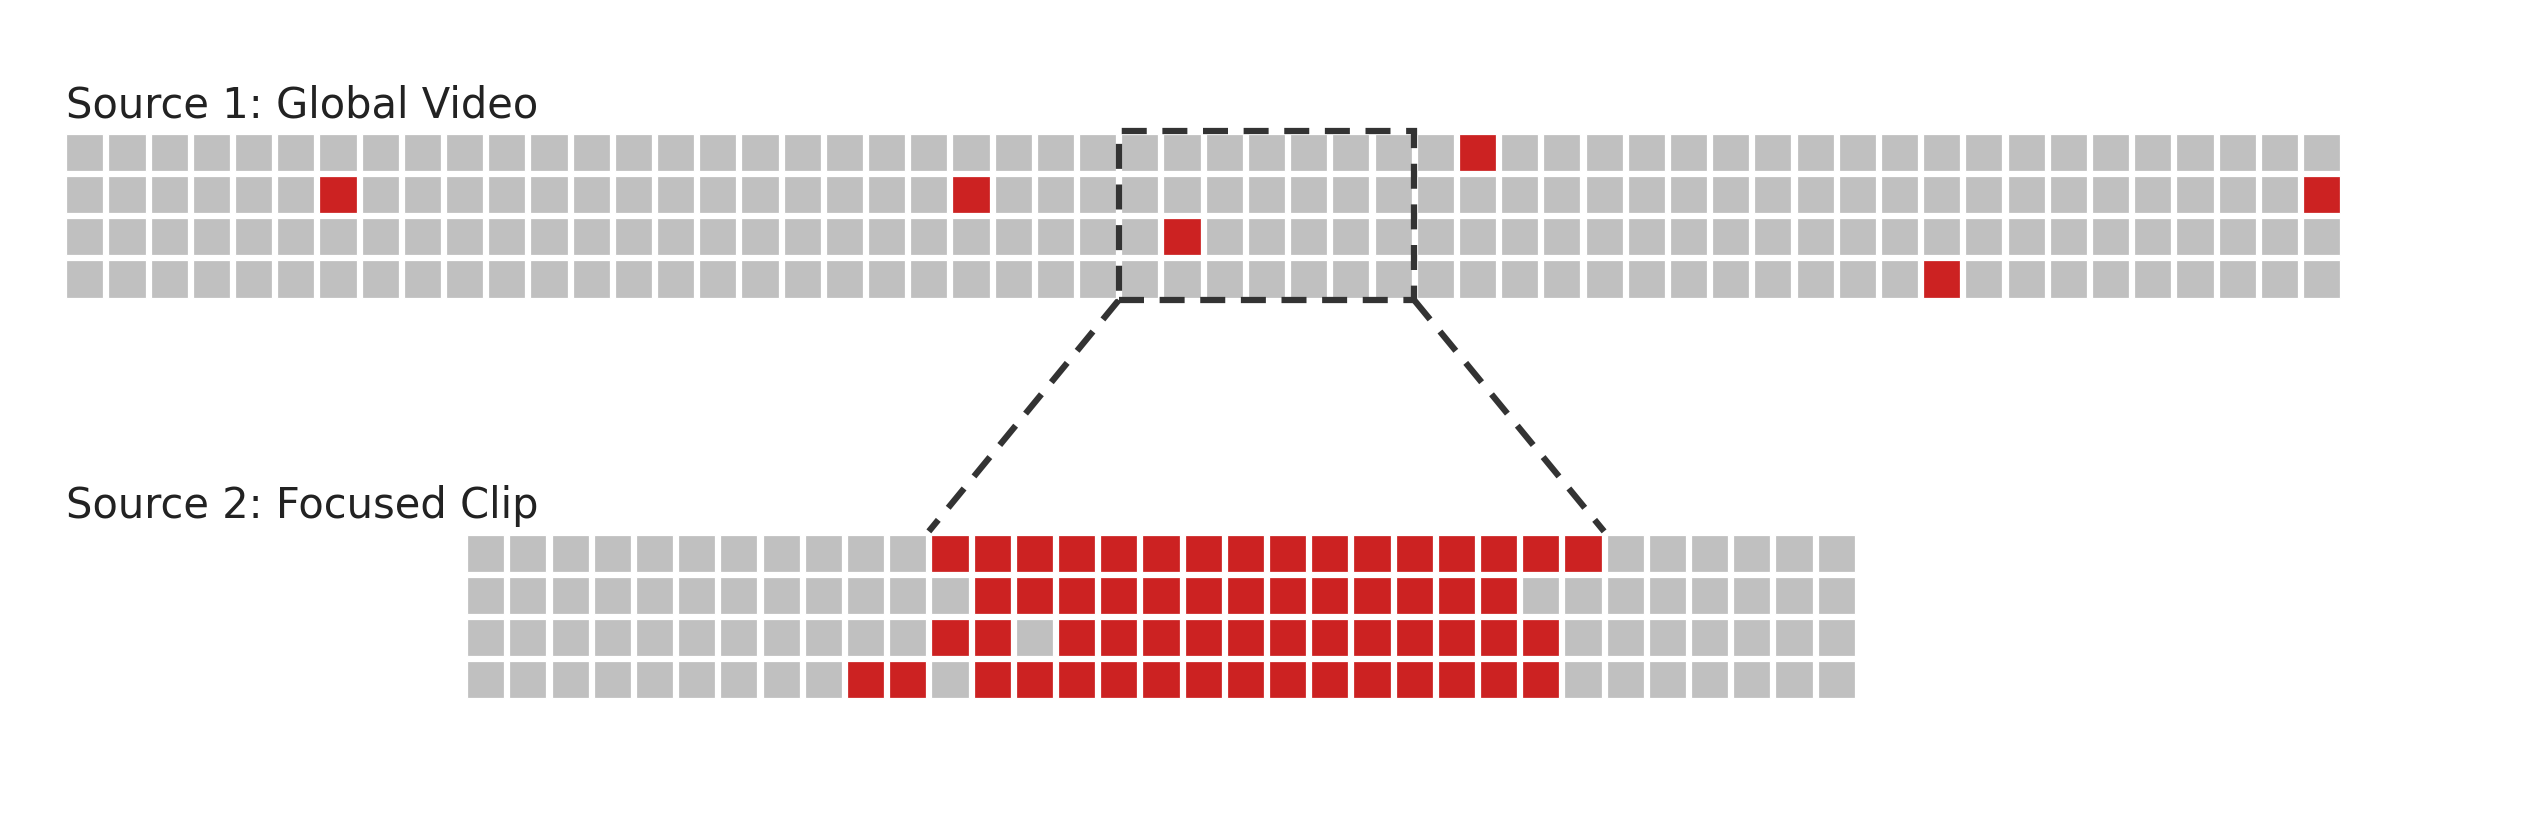
\includegraphics[width=\columnwidth]{figures/fig_temporal_zoomin.png}
  \caption{Temporal Zoom-in effect. Source~1 is the complete video; the small squares denote temporally sampled frames/visual tokens distributed over its full timeline, not object proposals. Source~2 is a clip cut from the Scout candidate window and sampled separately. In this example, the annotated anomaly occupies $\sim$1.6\% of Source~1 but $\sim$13.3\% of Source~2. Both sources are jointly provided to Sniper.}
  \label{fig:temporal_zoom}
\end{figure}

\subsection{Interaction-Aware Reasoning Prompt}
\label{sec:prompt}

To encourage explicit verification, we use a three-step structured reasoning prompt~\cite{wang2022self,yao2023tree}:


(1) \textbf{Observation}: Describe micro-actions in Source~2 (hand movements, body language).
(2) \textbf{Context Analysis}: Use Source~1 to identify environment and behavioral norms.
(3) \textbf{Classification}: Match against known anomaly patterns, explicitly \textbf{ruling out alternative benign explanations} (e.g., ``play fighting'' vs. ``assault'').

Compared to full video repetition ($V \oplus V$), ATR only repeats a short critical segment
($V \oplus \delta$); token overhead and efficiency comparisons are detailed in
Section~\ref{sec:discussion}.


\section{Experiments}
\label{sec:experiments}

\subsection{Experimental Setup}
\label{sec:setup}

\subsubsection{Datasets}

\textbf{Primary Dataset: UCF-Crime}~\cite{sultani2018real}. We use the official test partition (\textbf{290 videos}: 140 anomaly + 150 normal) for all primary results. We additionally report a full-pool evaluation (\textbf{1900 videos}: 950 anomaly + 950 normal, Section~\ref{sec:robustness}) as a separate robustness analysis. It uses only video-level normal/anomaly labels and does not assume frame-level ground truth for the training split. No full-pool sample is used for parameter updates or prompt fitting.
\textbf{Cross-Dataset Validation: XD-Violence}~\cite{wu2020not}. This dataset ($N$=800) presents a stringent modality gap test (high audio dependence) and higher native resolution, ideal for verifying ATR's spatio-temporal zoom-in capabilities.

\subsubsection{Models and Baselines}

We use \textbf{Qwen3-VL}~\cite{bai2025qwenvl} (4B, 8B, 32B) as the main controlled family because its open checkpoints provide multiple scales under a shared interface. We further test Qwen3.5-VL, the audio-visual Qwen2.5-Omni, and the \textbf{LLaVA-NeXT-Video-7B-Qwen2} architecture~\cite{li2024llavanext} (which uses a Qwen2 language backbone) to probe generational, modality, and framework transfer. Baselines include: (1) \textbf{Baseline (Global-Only)}: one call on the complete video; (2) \textbf{Clip-Only}: only the retrieved clip without global context; and (3) \textbf{ATR (Ours)}: Scout followed by a Sniper call that jointly receives the complete video and retrieved clip. We also report \textbf{Gemini 3.1 Pro}~\cite{team2023gemini} as a closed-source reference.
All inference uses deterministic decoding (\texttt{Temperature=0}). We evaluate three prompt strategies: \textbf{Aggressive} (safety-first, prefer false positives over missed detections), \textbf{Minimal} (concise with hallucination check), and \textbf{Neutral} (balanced, requires high confidence).
All videos are processed using the VLM's default temporal sampling strategy, which allocates frames proportional to source duration (e.g., $\sim$20 frames for a 2\,min video, $\sim$4 for a 15\,s clip). We deliberately retain this default without manual frame-count tuning to demonstrate that ATR's gains stem from temporal context focusing rather than increased sampling density.


\subsubsection{Evaluation Metrics}

We report \textbf{video-level} Accuracy, Precision, Recall, F1, False Negative Rate (FNR), and False Positive Rate (FPR). FNR is the fraction of anomaly videos predicted normal, while FPR is the fraction of normal videos predicted anomalous; reporting both exposes the operating-point trade-off hidden by accuracy alone. ATR does not output calibrated per-frame scores, so Frame-AUC, PR-AUC, mAP, and temporal IoU are not directly defined for its final output. These metrics remain appropriate for frame-level localization systems, but prior evaluations caution against using frame-level ranking as the only criterion for video-level decision quality and semantic understanding~\cite{doshi2022rethinking,zhang2024holmes,pi2024vader,chen2025ucvl}. We instead evaluate Scout's intermediate candidate quality separately in Section~\ref{sec:gt_scout}.

\subsection{Main Results}
\label{sec:main_results}

Table~\ref{tab:main} presents the core results on UCF-Crime.

\begin{table}[t]
  \small
  \centering
  \caption{Main results on UCF-Crime standard test set ($N$=290). \textbf{Bold}: best per
  method group. $\uparrow$/$\downarrow$: higher/lower is better.}
  \label{tab:main}
  \resizebox{\columnwidth}{!}{%
  \begin{tabular}{lcccccc}
    \toprule
    Method & Acc$\uparrow$ & Prec$\uparrow$ & Rec$\uparrow$ & F1$\uparrow$ & FPR$\downarrow$ & FNR$\downarrow$ \\
    \midrule
    \multicolumn{7}{l}{\textit{4B + Minimal (Primary Configuration)}} \\
    Baseline & 83.45\% & 90.35\% & 73.57\% & 81.10\% & 7.33\% & 26.43\% \\
    Clip-Only & 53.10\% & 83.33\% & 3.57\% & 6.85\% & 0.67\% & 96.43\% \\
    \textbf{ATR (Ours)} & \textbf{85.17\%} & 82.12\% & \textbf{88.57\%} & \textbf{85.22\%} & 18.00\% & \textbf{11.43\%} \\
    \midrule
    \multicolumn{7}{l}{\textit{8B + Aggressive (Secondary Configuration)}} \\
    Baseline & 82.41\% & 94.06\% & 67.86\% & 78.84\% & 4.00\% & 32.14\% \\
    Clip-Only & 71.03\% & 87.84\% & 46.43\% & 60.75\% & 6.00\% & 53.57\% \\
    \textbf{ATR (Ours)} & \textbf{85.52\%} & 88.89\% & \textbf{80.00\%} & \textbf{84.21\%} & 9.33\% & \textbf{20.00\%} \\
    \midrule
    \multicolumn{7}{l}{\textit{32B + Neutral (Upper Bound Reference)}} \\
    Baseline & 83.45\% & 80.26\% & 87.14\% & 83.56\% & 20.00\% & 12.86\% \\
    Clip-Only & 63.79\% & 100.00\% & 25.00\% & 40.00\% & 0.00\% & 75.00\% \\
    ATR (Ours) & 82.76\% & 81.25\% & 83.57\% & 82.39\% & 18.00\% & 16.43\% \\
    \bottomrule
  \end{tabular}}
\end{table}

In terms of accuracy, both 4B+ATR (85.17\%) and 8B+ATR (85.52\%) surpass the 32B Baseline (83.45\%), indicating that structured visual context can be a more efficient lever than raw parameter count. The primary benefit is recall: under 4B+Minimal, FNR drops from 26.43\% to 11.43\% (15.00 points), but FPR rises from 7.33\% to 18.00\%. The 8B+Aggressive configuration is more balanced: FNR decreases by 12.14 points while FPR increases by 5.33 points to 9.33\%. We therefore treat prompt/model selection as a deployment operating point, not a universal optimum. Meanwhile, Clip-Only's 96.43\% FNR confirms that local evidence without the complete video is insufficient. McNemar's test on the separate 1{,}900-video robustness pool confirms that the FNR reduction is significant ($p < 0.001$) for both model scales (Section~\ref{sec:robustness}).





\begin{figure}[h]
  \centering
  \includegraphics[width=\columnwidth]%\columnwidth,height=5.5cm,keepaspectratio]
  {figures/fig_category_breakdown.pdf}
  \caption{Per-category recall: Baseline vs.\ ATR (4B + Minimal, UCF-Crime $N$=290). Sorted by ATR$-$Baseline delta.}
  %Categories sorted by ATR$-$Baseline delta.}
  \label{fig:category}
\end{figure}

ATR delivers the largest gains in categories characterized by \textbf{transient or subtle visual cues}: Shoplifting (+33\%, $n$=21), RoadAccidents (+17\%, $n$=23), and Explosion (+14\%, $n$=21). In these scenarios, the anomaly occupies a tiny fraction of the spacetime volume. ATR's temporal zoom-in effectively amplifies these signals. The sole category exhibiting a decline is Arrest ($n$=5), where the small sample size precludes statistical significance.

\subsection{Cross-Scale Model Comparison}
\label{sec:cross_scale}

\begin{table}[t]
  \centering
  \caption{Per-model best prompt: Baseline vs.\ ATR (UCF-Crime $N$=290). Each model is paired with its best-performing prompt; please refer to Table~\ref{tab:prompt_ablation} for more details.}
  \label{tab:cross_scale}
  \resizebox{\columnwidth}{!}{%
  \begin{tabular}{llcccccc}
    \toprule
    Model & Prompt & BL Acc & ATR Acc & $\Delta$ Acc & BL FNR & ATR FNR & $\Delta$ FNR \\
    \midrule
    \textbf{4B} & Minimal & 83.45\% & \textbf{85.17\%} & \textbf{+1.72\%} & 26.43\% & \textbf{11.43\%} & \textbf{$-$15.00\%} \\
    \textbf{8B} & Aggressive & 82.41\% & \textbf{85.52\%} & \textbf{+3.11\%} & 32.14\% & \textbf{20.00\%} & \textbf{$-$12.14\%} \\
    32B & Neutral & 83.45\% & 82.76\% & $-$0.69\% & 12.86\% & 16.43\% & +3.57\% \\
    \bottomrule
  \end{tabular}}
\end{table}

The negative gain on 32B ($-$0.69\%) is analyzed in Section~\ref{sec:over_alignment}: its Scout retrieves fewer candidate intervals and its Sniper is more conservative on close-up evidence. The 4B configuration gives the lowest FNR (11.43\%), whereas the 8B configuration provides the lower-FPR operating point (9.33\%).

\subsection{Large-Scale Zero-Shot Robustness}
\label{sec:robustness}

To test distributional robustness beyond the official test partition, we evaluate on the full UCF-Crime pool ($N$=1900) using video-level labels only. This is an additional analysis, not a replacement for the official test protocol and not a frame-level benchmark.

\begin{table}[t]
  \centering
  \caption{Standard test set ($N$=290) vs.\ full dataset pool ($N$=1900): key configurations.}
  \label{tab:robustness}
  \resizebox{\columnwidth}{!}{%
  \begin{tabular}{llcccc}
    \toprule
    Config & Metric & \multicolumn{2}{c}{Test Set ($N$=290)} & \multicolumn{2}{c}{Full Pool ($N$=1900)} \\
    \cmidrule(lr){3-4}\cmidrule(lr){5-6}
    & & BL & ATR & BL & ATR \\
    \midrule
    \multirow{3}{*}{4B+Min} & Acc$\uparrow$ & 83.45\% & \textbf{85.17\%} & 84.05\% & \textbf{85.26\%} \\
    & FNR$\downarrow$ & 26.43\% & \textbf{11.43\%} & 26.95\% & \textbf{14.32\%} \\
    & FPR$\downarrow$ & 7.33\% & 18.00\% & 4.95\% & 15.16\% \\
    \midrule
    \multirow{3}{*}{8B+Agg} & Acc$\uparrow$ & 82.41\% & \textbf{85.52\%} & 83.11\% & \textbf{85.00\%} \\
    & FNR$\downarrow$ & 32.14\% & \textbf{20.00\%} & 31.05\% & \textbf{20.53\%} \\
    & FPR$\downarrow$ & 4.00\% & 9.33\% & 2.74\% & 9.47\% \\
    \midrule
    \multirow{3}{*}{32B+Neu} & Acc$\uparrow$ & \textbf{83.45\%} & 82.76\% & \textbf{86.26\%} & 80.58\% \\
    & FNR$\downarrow$ & \textbf{12.86\%} & 16.43\% & \textbf{13.26\%} & 35.26\% \\
    & FPR$\downarrow$ & 20.00\% & 18.00\% & 14.21\% & 3.58\% \\
    \bottomrule
  \end{tabular}}
\end{table}

The performance of 4B+ATR remains stable (Acc 85.26\%, FNR 14.32\%) at 6.5$\times$ scale, confirming robustness. In contrast, the 32B model's degradation intensifies on the full set ($-$5.68\% vs.\ $-$0.69\%), reinforcing the Over-Alignment hypothesis: the model's Scout conservatism is particularly acute on the more challenging full dataset.

\textbf{Statistical Significance}. McNemar's test on the full 1{,}900-video pool confirms that ATR's FNR reduction is highly significant for both 4B and 8B ($p < 0.001$): under 4B, ATR correctly detects 147 anomaly videos missed by Baseline while losing only 23; under 8B, the counts are 126 vs.\ 25. The overall accuracy gain is significant for 8B ($p = 0.017$) but not for 4B ($p = 0.23$), because ATR's FPR increase partially offsets the FNR improvement in the aggregate metric.

\subsection{Qualitative Case Study}
\label{sec:qualitative}

Figure~\ref{fig:qualitative} illustrates the reasoning process for \emph{Shooting007}. \textbf{Baseline} outputs only ``Answer: No,'' as the shooting occupies a negligible fraction of the 48\,s footage. \textbf{Clip-Only} judges ``normal activity\ldots no evidence of a threat,'' lacking global context to interpret a running person as flight. \textbf{ATR} fuses the global setting (backyard) with the local detail (urgent running) and correctly flags the anomaly: ``Rapid movement across the yard is unusual\ldots possibly fleeing or being chased.''

\begin{figure*}[t]
  \centering
  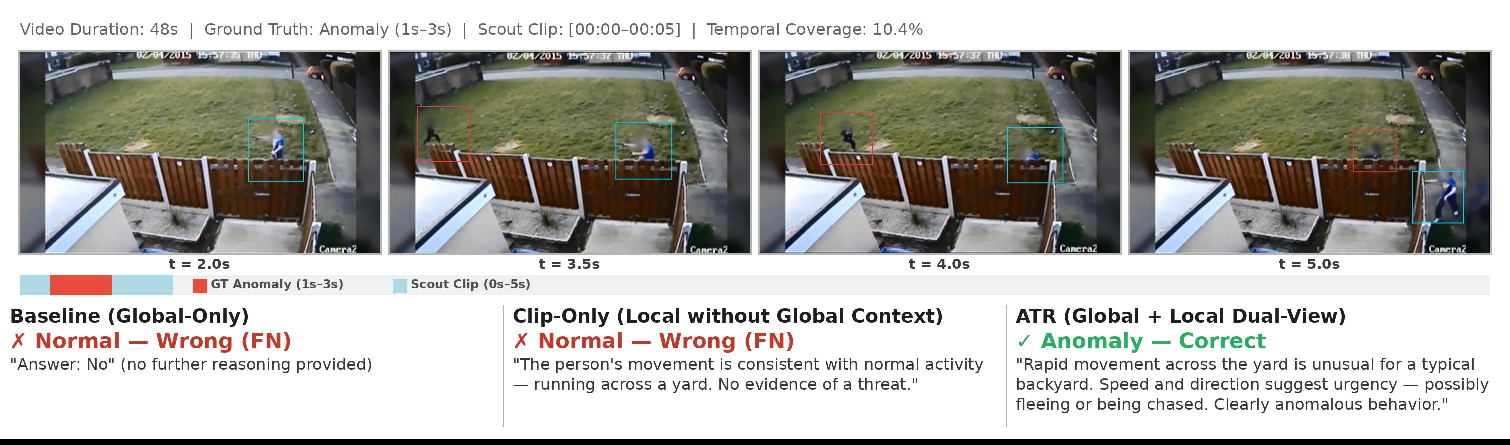
\includegraphics[width=\linewidth]{figures/fig_qualitative.pdf}
  \caption{Qualitative comparison on \emph{Shooting007}. ATR fuses global context (establishing the setting) with local detail (amplifying urgency cues), yielding a correct Anomaly classification where baselines fail.}
  \label{fig:qualitative}
\end{figure*}

\subsection{Cross-Paradigm Comparison}
\label{sec:cross_paradigm}

\begin{table}[t]
  \centering
  \caption{Cross-paradigm performance comparison on the UCF-Crime standard test set ($N$=290). ``--'' denotes an inapplicable metric. $\dagger$~LAVAD frame scores are max-aggregated per video and binarized with threshold $t$; $t{=}0.5$ is fixed, while oracle $t$ is selected post hoc on this evaluation set and is reported only as an upper-bound reference.}
  \label{tab:cross_paradigm}
  \resizebox{\columnwidth}{!}{%
  \begin{tabular}{lccccc}
    \toprule
    Method & Supervision & F.AUC$\uparrow$ & V.Acc$\uparrow$ & V.FNR$\downarrow$ & V.FPR$\downarrow$ \\
    \midrule
    LAVAD\textsuperscript{$\dagger$} ($t$=0.5)~\cite{zanella2024harnessing} & Training-Free & 80.28\% & 67.59\% & 63.57\% & 3.33\% \\
    LAVAD\textsuperscript{$\dagger$} (oracle $t$)~\cite{zanella2024harnessing} & Training-Free & 80.28\% & 82.76\% & 22.14\% & 12.67\% \\
    Gemini 3.1 Pro~\cite{team2023gemini} & Zero-Shot & -- & 73.10\% & 6.43\% & 46.00\% \\
    \textbf{ATR (Qwen3-VL-4B)} & \textbf{Zero-Shot} & -- & \textbf{85.17\%} & \textbf{11.43\%} & \textbf{18.00\%} \\
    \textbf{ATR (Qwen3-VL-8B)} & \textbf{Zero-Shot} & -- & \textbf{85.52\%} & \textbf{20.00\%} & \textbf{9.33\%} \\
    \bottomrule
  \end{tabular}}
\end{table}

Gemini 3.1 Pro obtains low FNR but a 46.00\% FPR under our zero-shot prompt, illustrating why accuracy, FNR, and FPR must be interpreted together. ATR's 4B and 8B operating points achieve higher accuracy with substantially lower FPR in this protocol. We do not mix these video-level results with weakly supervised frame-level SOTA rankings because the supervision, output granularity, and metrics differ.

\subsection{Cross-Dataset Generalization: XD-Violence}
\label{sec:xd_violence}

\begin{table}[t]
  \centering
  \caption{XD-Violence per-model best prompt: Baseline vs.\ ATR ($N$=800).}
  \label{tab:xd_best}
  \resizebox{\columnwidth}{!}{%
  \begin{tabular}{llcccccc}
    \toprule
    Model & Prompt & BL Acc & ATR Acc & $\Delta$ Acc & BL FNR & ATR FNR & $\Delta$ FNR \\
    \midrule
    4B & Minimal & 34.12\% & \textbf{49.00\%} & \textbf{+14.88\%} & 67.27\% & \textbf{48.53\%} & \textbf{$-$18.74\%} \\
    8B & Aggressive & 42.38\% & \textbf{50.75\%} & \textbf{+8.37\%} & 54.97\% & \textbf{46.57\%} & \textbf{$-$8.39\%} \\
    \bottomrule
  \end{tabular}}
\end{table}

Despite the lower absolute accuracy (a consequence of XD-Violence's heavy audio dependence, which disadvantages vision-only models), the relative improvement (+14.88\%) substantially exceeds that on UCF-Crime (+1.72\%), consistent with the greater headroom available when the baseline is weaker. This interpretation is further supported by the Qwen2.5-Omni experiment (Section~\ref{sec:omni}), where restoring the audio modality yields +29.33\% accuracy.


\subsection{Cross-Modal Validation: Qwen2.5-Omni on XD-Violence}
\label{sec:omni}

To further unlock ATR's potential through \textbf{spatio-temporal joint zoom-in}, we evaluate with Qwen2.5-Omni-7B~\cite{xu2025qwenomni} on XD-Violence. The global scan runs at 1~FPS while the Sniper clip runs at 2~FPS (Qwen2.5-Omni supports explicit frame-rate specification, unlike Qwen3-VL's duration-proportional allocation), producing a genuine physical frame-rate differential in addition to temporal window compression. Combined with native audio-visual joint reasoning, this activates all three amplification channels simultaneously.

\begin{table}[t]
  \centering
  \caption{Qwen2.5-Omni-7B on XD-Violence ($N$=800): 3 prompt styles.}
  \label{tab:omni}
  \resizebox{\columnwidth}{!}{%
  \begin{tabular}{lccccccc}
    \toprule
    Prompt & BL Acc & ATR Acc & $\Delta$ Acc & BL F1 & ATR F1 & BL FNR & ATR FNR \\
    \midrule
    \textbf{Minimal} & 38.42\% & \textbf{67.75\%} & \textbf{+29.33\%} & 53.50\% & \textbf{80.63\%} & 60.36\% & \textbf{24.90\%} \\
    Aggressive & 32.29\% & 54.44\% & +22.15\% & 47.83\% & 69.36\% & 65.27\% & 42.30\% \\
    Neutral & 28.54\% & 47.50\% & +18.96\% & 42.96\% & 62.16\% & 69.89\% & 51.75\% \\
    \bottomrule
  \end{tabular}}
\end{table}

Under full-modality conditions, Qwen2.5-Omni achieves substantial positive gains under \textbf{all three prompt styles} (+18.96\%--+29.33\% Accuracy), eliminating the prompt sensitivity observed in vision-only models. The Minimal configuration improves F1 from 53.50\% to 80.63\% (+27.13) and reduces FNR from 60.36\% to 24.90\% ($-$35.46\%). The larger gains compared to vision-only models (+29.33\% vs.\ +14.88\%) suggest that audio-visual joint reasoning provides a complementary amplification channel for ATR.


\subsection{Cross-Model-Family Validation: Qwen3.5-VL}
\label{sec:qwen35}

To evaluate whether ATR's observed patterns generalize beyond the Qwen3-VL family, we conduct experiments on the next-generation \textbf{Qwen3.5-VL-Instruct} series (9B and 27B) using the same UCF-Crime standard test set ($N$=290) and three prompt strategies. Thinking mode is disabled (\texttt{enable\_thinking=False}) to ensure outputs are directly comparable to Qwen3-VL experiments.

\begin{table}[t]
  \centering
  \caption{Qwen3.5-VL on UCF-Crime ($N$=290): Baseline vs.\ ATR.}
  \label{tab:qwen35}
  \resizebox{\columnwidth}{!}{%
  \begin{tabular}{llcccccc}
    \toprule
    Model & Prompt & BL Acc & ATR Acc & $\Delta$ Acc & BL FNR & ATR FNR & $\Delta$ FNR \\
    \midrule
    9B & Minimal & 86.90\% & 66.21\% & $-$20.69\% & 12.86\% & 30.00\% & +17.14\% \\
    9B & Aggressive & 81.72\% & 66.90\% & $-$14.83\% & 24.29\% & 11.43\% & $-$12.86\% \\
    9B & \textbf{Neutral} & 82.41\% & \textbf{85.52\%} & \textbf{+3.10\%} & 33.57\% & \textbf{21.43\%} & \textbf{$-$12.14\%} \\
    \midrule
    27B & Minimal & 85.17\% & 76.90\% & $-$8.28\% & 20.00\% & 31.43\% & +11.43\% \\
    27B & Aggressive & 84.48\% & 82.07\% & $-$2.41\% & 16.43\% & 19.29\% & +2.86\% \\
    27B & Neutral & 85.52\% & 83.45\% & $-$2.07\% & 14.29\% & 28.57\% & +14.28\% \\
    \bottomrule
  \end{tabular}}
\end{table}

Qwen3.5-9B achieves 86.90\% baseline accuracy (Minimal), already surpassing the best Qwen3-VL ATR result (8B+ATR, 85.52\%; Table~\ref{tab:cross_scale}). Only 9B+Neutral yields a positive ATR gain (+3.10\%); all other configurations show negative or marginal returns, consistent with the diminishing-returns pattern observed for Qwen3-VL~32B and analyzed in Section~\ref{sec:over_alignment}.

\subsection{Cross-Framework Validation: LLaVA-NeXT-Video}
\label{sec:llava_validation}

To test whether the observed gain is specific to the Qwen VLM interface, we evaluate LLaVA-NeXT-Video-7B-Qwen2 with a fixed aggressive prompt on the same UCF-Crime test set. Baseline and ATR use identical decoding and Yes/No parsing; the only protocol change is global-only input versus the full-video-plus-retrieved-clip Sniper input.

\begin{table}[t]
  \centering
  \caption{Cross-backbone check with LLaVA-NeXT-Video-7B-Qwen2 on UCF-Crime ($N$=290), using the same aggressive prompt for both methods.}
  \label{tab:llava_validation}
  \resizebox{\columnwidth}{!}{%
  \begin{tabular}{lcccccc}
    \toprule
    Method & Acc & Prec & Rec & F1 & FPR & FNR \\
    \midrule
    Global-Only & 72.76\% & 100.00\% & 43.57\% & 60.70\% & 0.00\% & 56.43\% \\
    \textbf{ATR} & \textbf{77.24\%} & 100.00\% & \textbf{52.86\%} & \textbf{69.16\%} & 0.00\% & \textbf{47.14\%} \\
    \bottomrule
  \end{tabular}}
\end{table}

ATR improves accuracy by 4.48 points and recall by 9.29 points without increasing FPR in this configuration. This matched-prompt comparison supports transfer of the input protocol beyond the main Qwen-VL implementation. The complete LLaVA-family sweep is mixed (Appendix Table~\ref{tab:llava_full}), so we describe ATR as framework-, backbone-, and alignment-sensitive rather than universally VLM-agnostic.


\section{Ablation Studies}
\label{sec:ablation}

\subsection{Module Effectiveness Ablation}
\label{sec:module_ablation}

\begin{table}[h]
  \small
  \centering
  \caption{Module ablation (UCF-Crime standard test set, $N$=290).}
  \label{tab:module_ablation}
  \begin{tabular}{llcccc}
    \toprule
    Config & Setting & Scout & Global & Acc & FNR \\
    \midrule
    \multirow{3}{*}{4B+Min} & A: Clip-Only & \checkmark & $\times$ & 53.10\% & 96.43\% \\
    & B: Baseline & $\times$ & \checkmark & 83.45\% & 26.43\% \\
    & \textbf{C: ATR (Full)} & \checkmark & \checkmark & \textbf{85.17\%} & \textbf{11.43\%} \\
    \midrule
    \multirow{3}{*}{8B+Agg} & A: Clip-Only & \checkmark & $\times$ & 71.03\% & 53.57\% \\
    & B: Baseline & $\times$ & \checkmark & 82.41\% & 32.14\% \\
    & \textbf{C: ATR (Full)} & \checkmark & \checkmark & \textbf{85.52\%} & \textbf{20.00\%} \\
    \bottomrule
  \end{tabular}
\end{table}

\textbf{Analysis}: Full ATR outperforms both Clip-Only and Baseline across all configurations,
confirming the necessity of dual-view fusion. Padding-direction robustness is reported separately in Table~\ref{tab:ace_ablation}; the performance gain is driven by the Scout--Sniper retrieval mechanism rather than a particular padding direction.
Critically, the gain is not attributable to token volume alone.
To isolate the source of improvement, we conduct a controlled input content ablation (Table~\ref{tab:input_content}) on 100 videos where Scout produced candidates (72 anomaly + 28 normal, 4B+Minimal).
All groups share the same global video, Sniper prompt, and separators; only Source~2 differs, with \textbf{duration matched} to the original Scout clip ($\sim$$L+\delta$ tokens each).

\begin{table}[t]
  \centering
  \caption{Input content ablation (4B+Minimal, 100 videos where Scout triggered: 72 anomaly + 28 normal). Only Source~2 content varies; global video, prompt, and token budget ($L+\delta$) are held constant.}
  \label{tab:input_content}
  \resizebox{\columnwidth}{!}{%
  \begin{tabular}{llcccc}
    \toprule
    Group & Source~2 Content & Acc$\uparrow$ & FNR$\downarrow$ & FPR$\downarrow$ \\
    \midrule
    A: Baseline & None (global only) & 71.0\% & 26.4\% & 35.7\% \\
    B: Unrelated & Different video, different category & 59.0\% & 19.4\% & 96.4\% \\
    C: Wrong Segment & Same-video non-Scout segment & 70.0\% & 2.8\% & 100.0\% \\
    \textbf{D: ATR (Ours)} & \textbf{Scout-retrieved candidate clip} & \textbf{72.0\%} & \textbf{1.4\%} & 96.4\% \\
    \bottomrule
  \end{tabular}}
\end{table}

Cross-video noise~(B) degrades accuracy by 12.0 points relative to Baseline, showing that added visual tokens alone do not explain the gain. The same-video wrong segment~(C) also fails to improve accuracy and drives FPR to 100.0\%, directly distinguishing ATR from arbitrary truncation. The Scout-retrieved clip~(D) gives the best accuracy and lowest FNR in this candidate-triggered subset. Because conditioning on Scout activation changes the class distribution and all local-view variants are recall-oriented, these FPR values are not deployment operating points; the complete 290-video FPR/FNR results are reported in Table~\ref{tab:main}.

\subsection{Temporal Context Padding Robustness}
\label{sec:ace_ablation}

\begin{table}[h]
  \centering
  \caption{Equal-budget temporal context padding on the frozen paired subset ($N=178$; 89 anomaly and 89 normal videos). All conditions reuse the same Scout candidates. Entries are balanced accuracy.}
  \label{tab:ace_ablation}
  \resizebox{\columnwidth}{!}{%
  \begin{tabular}{lcccc}
    \toprule
    Model & $0/0$ & $6/6$ & $10/2$ & $2/10$ \\
    \midrule
    4B+Min & 89.89\% & 90.45\% & \textbf{91.01\%} & \textbf{91.01\%} \\
    8B+Agg & 91.01\% & 91.57\% & \textbf{92.70\%} & \textbf{92.70\%} \\
    \bottomrule
  \end{tabular}}
\end{table}

\textbf{Analysis}:
Table~\ref{tab:ace_ablation} reports pre/post padding in seconds. The equal-budget $10/2$ and $2/10$ conditions are identical for both model scales, and their differences from $6/6$ are not statistically significant. We retain $10/2$ only as the frozen implementation setting; ATR does not rely on an asymmetric temporal mechanism.


\subsection{Prompt Strategy Ablation}
\label{sec:prompt_ablation}

\begin{table}[h]
  \centering
  \caption{Prompt strategy ablation (ATR, full 1900-video evaluation).}
  \label{tab:prompt_ablation}
  \resizebox{\columnwidth}{!}{%
  \begin{tabular}{llcccccc}
    \toprule
    Model & Prompt & Acc & Prec & Rec & F1 & FPR & FNR \\
    \midrule
    4B & Aggressive & 83.32\% & 94.39\% & 70.84\% & 80.94\% & 4.21\% & 29.16\% \\
    4B & \textbf{Minimal} & \textbf{85.26\%} & 84.97\% & \textbf{85.68\%} & \textbf{85.32\%} & 15.16\% & \textbf{14.32\%} \\
    4B & Neutral & 69.05\% & 99.18\% & 38.42\% & 55.39\% & 0.32\% & 61.58\% \\
    \midrule
    8B & \textbf{Aggressive} & \textbf{85.00\%} & \textbf{89.35\%} & \textbf{79.47\%} & \textbf{84.12\%} & 9.47\% & \textbf{20.53\%} \\
    8B & Minimal & 75.68\% & 75.21\% & 76.63\% & 75.91\% & 25.26\% & 23.37\% \\
    8B & Neutral & 69.26\% & 99.46\% & 38.74\% & 55.76\% & 0.21\% & 61.26\% \\
    \midrule
    32B & Minimal & 79.58\% & 83.37\% & 73.89\% & 78.35\% & 14.74\% & 26.11\% \\
    32B & Aggressive & 76.74\% & 71.67\% & 88.42\% & 79.17\% & 34.95\% & 11.58\% \\
    32B & \textbf{Neutral} & \textbf{80.58\%} & \textbf{94.76\%} & 64.74\% & \textbf{76.92\%} & \textbf{3.58\%} & 35.26\% \\
    \bottomrule
  \end{tabular}}
\end{table}

\textbf{Analysis}: Prompt effects are strongly model-dependent. The 4B model performs best with Minimal, while the 8B model performs best with Aggressive; Neutral is highly conservative for both lightweight models. These differences should not be interpreted as a universal scale law. Instead, prompt style changes the recall--FPR operating point and must be reported together with the model choice. For each lightweight model ($\leq$8B), at least one prompt yields a positive ATR gain over its matched Baseline, but the selected operating point remains deployment-specific.

\subsection{GT-Anchored Scout: Upper-Bound Analysis of Sniper}
\label{sec:gt_scout}

To disentangle the contributions of the Scout and Sniper stages, we replace Scout's output with \textbf{ground-truth temporal annotations}, providing Sniper with perfect anomaly windows. This yields an upper-bound estimate of ATR's potential if Scout were ideal, and directly measures Sniper's standalone reasoning quality.

For the 140 anomaly videos, we supply GT time intervals to Sniper; for the 150 normal videos, no GT clip exists, so GT-ATR reduces to Baseline.

\begin{table}[t]
  \centering
  \caption{GT-Anchored Scout: Baseline vs.\ Scout-ATR vs.\ GT-ATR on UCF-Crime ($N$=290: 140 anomaly + 150 normal). GT-ATR shares TN/FP with Baseline on normal videos.}
  \label{tab:gt_scout}
  \resizebox{\columnwidth}{!}{%
  \begin{tabular}{llccccc}
    \toprule
    Model & Method & TP & FN & Acc & FNR & F1 \\
    \midrule
    \multirow{3}{*}{4B+Min}
    & Baseline & 103 & 37 & 83.45\% & 26.43\% & 81.10\% \\
    & Scout-ATR & 124 & 16 & 85.17\% & 11.43\% & 85.22\% \\
    & \textbf{GT-ATR} & \textbf{138} & \textbf{2} & \textbf{95.52\%} & \textbf{1.43\%} & \textbf{95.50\%} \\
    \midrule
    \multirow{3}{*}{8B+Agg}
    & Baseline & 95 & 45 & 82.41\% & 32.14\% & 78.84\% \\
    & Scout-ATR & 112 & 28 & 85.52\% & 20.00\% & 84.21\% \\
    & \textbf{GT-ATR} & \textbf{121} & \textbf{19} & \textbf{91.38\%} & \textbf{13.57\%} & \textbf{90.64\%} \\
    \midrule
    \multirow{3}{*}{32B+Neu}
    & Baseline & 122 & 18 & 83.45\% & 12.86\% & 83.56\% \\
    & Scout-ATR & 117 & 23 & 82.76\% & 16.43\% & 82.39\% \\
    & GT-ATR & 100 & 40 & 75.86\% & 28.57\% & 74.07\% \\
    \bottomrule
  \end{tabular}}
\end{table}

\textbf{Analysis}:
(1)~\textbf{Candidate evidence quality provides substantial headroom}: Under GT conditions, 4B achieves 95.52\% accuracy with only 2 missed detections out of 140 anomaly videos (FNR 1.43\%), and 8B reaches 91.38\%. The gap between Scout-ATR and GT-ATR (+10.35\% and +5.86\% respectively) quantifies the headroom available if the retrieved temporal evidence is improved. It does not imply that Scout is already a calibrated frame-level localizer.
(2)~\textbf{Close-up conservatism in 32B}: Even with perfect GT windows, 32B accuracy \emph{drops} from 83.45\% to 75.86\% ($-$7.59\%). On anomaly videos alone, 32B recall falls from 87.14\% (Baseline) to 71.43\% (GT-ATR), indicating that the model classifies focused anomaly clips as normal more often than when viewing only the global video. Per-category analysis reveals the sharpest degradation on visually violent categories (RoadAccidents: 82.61\%$\rightarrow$39.13\%; Abuse: 100\%$\rightarrow$50\%), suggesting that the 32B Sniper's safety alignment may actively suppress anomaly recognition when presented with close-up evidence of sensitive content.
(3)~Combined with Scout-stage conservatism (Section~\ref{sec:over_alignment}), these results reveal a \textbf{dual-stage compounding failure} for 32B that explains its consistently negative ATR gains.

\subsection{Scout--GT Temporal Offset Diagnostic}
\label{sec:scout_offset}

The GT-anchored experiment measures an upper bound but not how free-form Scout timestamps align with the annotated core action. For each of the 140 anomaly videos in the standard test set, we select the Scout candidate nearest to any official GT interval and compute their signed temporal relation. A negative distance means the candidate ends before the GT interval; a positive distance means it starts after the GT interval. Percentages below are conditioned on anomaly videos where Scout returned at least one candidate.

\begin{table}[t]
  \centering
  \caption{Scout candidate position relative to the nearest official GT interval. ``Before/overlap/after'' uses the original Scout timestamps.}
  \label{tab:scout_offset}
  \resizebox{\columnwidth}{!}{%
  \begin{tabular}{lccccc}
    \toprule
    Config & Candidate videos & Before & Overlap & After & Median gap \\
    \midrule
    4B+Minimal & 126/140 & 91.3\% & 8.7\% & 0.0\% & $-$17.25\,s \\
    8B+Aggressive & 138/140 & 91.3\% & 8.7\% & 0.0\% & $-$17.00\,s \\
    32B+Neutral & 95/140 & 90.5\% & 9.5\% & 0.0\% & $-$21.00\,s \\
    \bottomrule
  \end{tabular}}
\end{table}

The offset is strongly directional rather than randomly distributed before and after the GT interval. Expanding Scout windows with the fixed contextual padding raises strict overlap to 13.5\%, 13.8\%, and 15.8\% for 4B, 8B, and 32B, respectively. This pattern is consistent with Scout often selecting pre-event context or assigning an early timestamp relative to the dataset's core-action annotation. It is not causal proof, and the low strict-overlap rates confirm that Scout timestamps should not be interpreted as precise temporal boundaries. Accordingly, our primary claim concerns semantic evidence retrieval for downstream video-level decisions, with GT-ATR serving as the candidate-quality upper bound.


\section{Discussion}
\label{sec:discussion}

\subsection{Efficiency: The ``Framework-for-Compute'' Strategy}

ATR demonstrates that intelligent retrieval can substitute for raw model scale. As shown in Table~\ref{tab:efficiency_compare}, both 4B+ATR and 8B+ATR surpass the 32B Baseline in accuracy while running on a single consumer GPU (RTX 4090) at $\leq$10\% of the 32B's GPU$\cdot$h cost (8$\times$ A100).

\begin{table}[t]
  \centering
  \caption{Efficiency: ATR configurations vs.\ 32B Baseline (1$\times$ RTX~4090 unless noted).}
  \label{tab:efficiency_compare}
  \resizebox{\columnwidth}{!}{%
  \begin{tabular}{lccccc}
    \toprule
    Config & GPUs & GPU$\cdot$h & s/video & Acc & FNR \\
    \midrule
    32B Baseline & 8$\times$ A100 & 92.6 & 22.0 & 83.45\% & 12.86\% \\
    \textbf{8B+ATR} & 1$\times$ RTX~4090 & \textbf{7.4} & \textbf{14.0} & \textbf{85.52\%} & 20.00\% \\
    \textbf{4B+ATR} & 1$\times$ RTX~4090 & 9.0 & 17.1 & 85.17\% & \textbf{11.43\%} \\
    \bottomrule
  \end{tabular}}
\end{table}

This gain is not due to token volume. ATR adds only $\sim$5\% input tokens ($\sim$59 tokens) over Baseline (Table~\ref{tab:efficiency}), yet reduces FNR by 12.63\% absolute. This confirms that the performance leap stems from the \textbf{quality of information} (targeted visual content) rather than the quantity of tokens.

\begin{table}[t]
  \centering
  \caption{Token overhead (4B+Minimal, full 1900-video run, avg.\ input tokens).}
  \label{tab:efficiency}
  \resizebox{\columnwidth}{!}{%
  \begin{tabular}{lccccc}
    \toprule
    Method & Input & Avg Tokens & Acc & FNR & FPR \\
    \midrule
    Baseline & $[V,Q]$ & $\sim$1,208 & 84.05\% & 26.95\% & 4.95\% \\
    Clip-Only & $[V_\text{clip},Q]$ & $\sim$600 & 52.32\% & 95.26\% & 0.11\% \\
    \textbf{ATR (Ours)} & $[V,V_\text{clip},Q]$ & $\sim$\textbf{1,267} & \textbf{85.26\%} & \textbf{14.32\%} & 15.16\% \\
    \bottomrule
  \end{tabular}}
\end{table}

\subsection{The Over-Alignment Phenomenon}
\label{sec:over_alignment}

The 32B model exhibits negative ATR gains ($-$0.69\% on the test set; $-$5.68\% on the full 1900-video pool). We analyze this as a \textbf{dual-stage degradation pattern} that is consistent with conservative alignment behavior, while acknowledging that the present experiments do not isolate safety alignment as the sole causal factor~\cite{ouyang2022training}.

\textbf{Scout-stage conservatism.}
The 32B Scout's failure rate on anomaly videos (30.5\%) consistently exceeds that of 4B (12.8\%) and 8B (3.4\%) under their respective best prompts, with concealed categories most affected (Table~\ref{tab:scout_category}: Shoplifting 56.0\%, RoadAccidents 52.7\%). Yet when Scout \emph{does} succeed, 32B's Sniper de-escalation rate is the \emph{lowest} (7.1\% vs.\ 50.4\%/48.4\% for 4B/8B), indicating a ``candidate conservatism + verification stability'' pattern consistent with, but not uniquely explained by, stronger alignment~\cite{rottger2024xstest,askell2021general}.

\begin{table}[t]
  \centering
  \caption{Scout failure rate (\%) by anomaly category under each model's best prompt (full 1900-video evaluation).}
  \label{tab:scout_category}
  \resizebox{\columnwidth}{!}{%
  \begin{tabular}{lccc}
    \toprule
    Category & 4B+Min & 8B+Agg & 32B+Neu \\
    \midrule
    Shoplifting ($n$=50)     & 24.0 & 0.0  & \textbf{56.0} \\
    RoadAccidents ($n$=150)  & 23.3 & 7.3  & \textbf{52.7} \\
    Abuse ($n$=50)           & 18.0 & 2.0  & \textbf{40.0} \\
    Burglary ($n$=100)       & 8.0  & 1.0  & 34.0 \\
    Shooting ($n$=50)        & 0.0  & 0.0  & 30.0 \\
    Stealing ($n$=100)       & 7.0  & 1.0  & 29.0 \\
    Vandalism ($n$=50)       & 6.0  & 2.0  & 26.0 \\
    Explosion ($n$=50)       & 12.0 & 8.0  & 24.0 \\
    Robbery ($n$=150)        & 7.3  & 0.0  & 20.7 \\
    \bottomrule
  \end{tabular}}
\end{table}

\textbf{Sniper-stage close-up conservatism.}
The GT-anchored ablation (Section~\ref{sec:gt_scout}) reveals a second layer: given perfect temporal windows, 32B's anomaly-video recall \emph{drops} from 87.14\% to 71.43\% (RoadAccidents: 82.61\%$\rightarrow$39.13\%), whereas 4B and 8B dramatically \emph{improve} (4B: 73.57\%$\rightarrow$98.57\%). The 32B model thus under-detects at Scout \emph{and} under-classifies at Sniper, compounding into consistently negative ATR gains. These results highlight a practical tension between safety alignment and domain-specific anomaly perception. Cross-family validation on Qwen3.5-VL (Section~\ref{sec:qwen35}) confirms this pattern extends beyond a single model series.

\label{sec:boundaries}
\textbf{Applicability boundaries.} These findings converge on three regimes: \textbf{Effective} for selected lightweight-model operating points; \textbf{Diminishing returns} as the baseline saturates through scaling or generational improvement; and \textbf{Adverse} for some larger or conservative models. The positive LLaVA-NeXT result (Section~\ref{sec:llava_validation}) shows that ATR is not tied to one inference interface, but the mixed Qwen3.5 and wider LLaVA-family results rule out a universal model-agnostic claim. ATR is thus a \textbf{compute-efficient strategy for bridging the gap between lightweight and large models}, rather than a universal enhancer.

\subsection{Limitations}

First, Scout is a semantic candidate retriever rather than a calibrated frame-level localizer. Its timestamps frequently precede the official core-action interval (Section~\ref{sec:scout_offset}), and a missed candidate cannot be recovered by Sniper; the global-only fallback is conservative rather than corrective. Second, ATR shifts the FNR/FPR operating point. The 4B configuration prioritizes recall and increases FPR, while the 8B setting is more balanced; both metrics must be reported for deployment. Third, gains depend on prompt style, backbone sensitivity, and alignment. Generic VLM pretraining also leaves a domain gap for low-resolution surveillance footage, so absolute reliability should not be assumed without domain-specific validation. Finally, the full 1{,}900-video result is a video-level robustness analysis only; primary benchmark claims remain on the official 290-video test split.


\section{Conclusion}
\label{sec:conclusion}

We presented Anomaly-Targeted Retrieval (ATR), a training-free framework for content-relevant intra-video retrieval. Scout scans the complete video, and Sniper then jointly receives the same complete video and a retrieved local clip; ATR is therefore global--local reasoning rather than local-only truncation. On UCF-Crime, ATR enables a 4B model to reach 85.17\% accuracy and an 8B model to reach 85.52\%, outperforming a 32B baseline (83.45\%) at $\sim$10\% of its GPU-hour cost. The gains arise mainly from fewer missed anomalies and must be interpreted with the accompanying FPR trade-off. Cross-dataset, audio-visual, and LLaVA-NeXT experiments show transfer beyond the primary Qwen setup, while prompt and backbone sensitivity define clear applicability boundaries. GT-ATR quantifies substantial headroom from better candidate evidence, whereas the offset diagnostic confirms that Scout should not be described as a calibrated frame-level localizer. ATR is therefore a compute-efficient operating strategy for selected lightweight VLMs, not a universal model enhancer.

% We have presented \textbf{Anomaly-Targeted Retrieval (ATR)}, a training-free framework that reconciles the fundamental tension between local sensitivity and global context in long-form video understanding. By formulating anomaly detection as an \textbf{Intra-Video Retrieval} problem, ATR introduces \textbf{Hierarchical Visual Repetition}---a Video-domain Visual RAG paradigm---to achieve efficient heterogeneous dual-view reasoning. This design preserves bidirectional attention benefits while reducing computational complexity from $O((2L)^2)$ to $O((L+\delta)^2)$.

% On the UCF-Crime standard test set ($N$=290), ATR effectively empowers lightweight models: the 4B model reduces FNR from 26.43\% to 11.43\% (relative reduction 56.8\%), achieving 85.17\% video-level accuracy. The 8B model with ATR reaches 85.52\%, surpassing the 32B Baseline (83.45\%) at approximately 8\% of the GPU$\cdot$h cost. ATR improves recall in 10 out of 13 anomaly categories, with the most substantial gains in concealed anomaly scenarios (Shoplifting +33\%). Large-scale robustness evaluation on the full 1,900-video pool confirms these findings.

% Crucially, ATR's efficacy extends beyond single-domain boundaries. Cross-dataset evaluation on XD-Violence ($N$=800) demonstrates consistent generalization. Furthermore, experiments with the multimodal Qwen2.5-Omni-7B show that ATR transfers seamlessly to audio-visual joint reasoning, achieving a massive F1 improvement from 53.50\% to 80.63\% (+27.13) and substantially breaking through the vision-only modality gap ceiling.

% Furthermore, we identify an \textbf{Over-Alignment Phenomenon} where the 32B model exhibits negative gains under ATR, revealing a critical trade-off between safety alignment and surveillance utility. Our findings provide a critical counter-evidence to the prevailing "scale-is-all-you-need" doctrine in safety-critical domains, demonstrating that lightweight models with targeted retrieval offer a superior efficiency-safety trade-off. By democratizing high-performance video understanding on consumer-grade hardware, ATR paves the way for scalable, privacy-preserving edge surveillance systems.


\appendix
\section{Method details}
% \section{Full Prompt Texts}
\label{sec:appendix_prompts}

This section provides the complete prompt texts used in our experiments. Three prompt strategies are evaluated: \textbf{Minimal}, \textbf{Aggressive}, and \textbf{Neutral}. Each strategy defines prompts for three modules: Baseline (global-only inference), Scout (temporal scanning), and Sniper (dual-view reasoning).

\subsection{Separator Texts (Sniper Input Construction)}

When constructing the Sniper's dual-view input, two separator texts are inserted between the video sources:

\begin{small}
\begin{verbatim}
[Sep_1] SOURCE 1: Global Context (Low FPS).
Use this ONLY to understand the setting
(e.g., store, street).

[Sep_2] SOURCE 2: Local Detail (High FPS,
Focused Clip). This clip contains the
CRITICAL MOMENT.
\end{verbatim}
\end{small}

\subsection{Minimal Strategy}

\subsubsection{Baseline Prompt (Minimal)}
\begin{small}
\begin{verbatim}
Is there any anomalous event or security
concern in this video?

Answer: Yes or No.
\end{verbatim}
\end{small}

\subsubsection{Scout Prompt (Minimal)}
\begin{small}
\begin{verbatim}
Analyze the entire video. Identify all
potential anomalies or suspicious events.
For each, provide:
- start and end timestamps (MM:SS)
- brief reason
- confidence (high/medium/low)

Return JSON:
[{"start":"MM:SS","end":"MM:SS",
  "reason":"...","confidence":"high"}]

If nothing suspicious, return: []
\end{verbatim}
\end{small}

\subsubsection{Sniper Prompt (Minimal)}
\begin{small}
\begin{verbatim}
Based on the two video sources provided:
Is there any anomalous event or security
concern?

Answer: Yes or No.
\end{verbatim}
\end{small}

\subsection{Aggressive Strategy}

\subsubsection{Baseline Prompt (Aggressive)}
\begin{small}
\begin{verbatim}
You are a surveillance video analyst.
Carefully watch the entire video and
determine whether it contains any
anomalous or criminal activity.

Consider these categories: Abuse, Arrest,
Arson, Assault, Burglary, Explosion,
Fighting, Road Accidents, Robbery,
Shooting, Shoplifting, Stealing,
Vandalism.

Provide your analysis:
1. Describe what you observe
2. Identify any suspicious activities
3. Final answer: "Answer: Yes" or
   "Answer: No"

Important: Even subtle or brief anomalies
should be flagged. Err on the side of
caution.
\end{verbatim}
\end{small}

\subsubsection{Scout Prompt (Aggressive)}
\begin{small}
\begin{verbatim}
You are a surveillance video analyst
performing temporal anomaly scanning.

Watch the ENTIRE video carefully and
identify ALL segments that contain or
suggest anomalous activity. Be thorough
and flag even subtle suspicious moments.

For each suspicious segment, provide:
- Precise start and end timestamps (MM:SS)
- Detailed description of the anomaly
- Confidence level (high/medium/low)
- Anomaly category if identifiable

Return as JSON array:
[{"start":"MM:SS","end":"MM:SS",
  "reason":"detailed description",
  "confidence":"high/medium/low",
  "category":"optional category"}]

If genuinely nothing suspicious: []

IMPORTANT: It is better to over-report
than to miss a real anomaly.
\end{verbatim}
\end{small}

\subsubsection{Sniper Prompt (Aggressive)}
\begin{small}
\begin{verbatim}
You are a surveillance video analyst
performing focused anomaly verification.

You are given TWO video sources:
- SOURCE 1: Full video (global context)
- SOURCE 2: A specific clip flagged as
  potentially anomalous

Your task:
1. Use SOURCE 1 to understand the overall
   scene and context
2. Carefully examine SOURCE 2 for any
   anomalous or criminal activity
3. Consider: Abuse, Arrest, Arson,
   Assault, Burglary, Explosion, Fighting,
   Road Accidents, Robbery, Shooting,
   Shoplifting, Stealing, Vandalism

Provide your analysis:
1. Scene context from SOURCE 1
2. Detailed analysis of SOURCE 2
3. Final verdict: "Answer: Yes" or
   "Answer: No"

Important: Even subtle anomalies should
be flagged. The clip was pre-selected as
suspicious -- examine it carefully.
\end{verbatim}
\end{small}

\subsection{Neutral Strategy}

\subsubsection{Baseline Prompt (Neutral)}
\begin{small}
\begin{verbatim}
Watch this video and determine whether it
contains any anomalous event.

Provide a brief explanation of your
reasoning, then give your final answer.

Answer: Yes or No.
\end{verbatim}
\end{small}

\subsubsection{Scout Prompt (Neutral)}
\begin{small}
\begin{verbatim}
Watch the video and identify any segments
that may contain unusual or anomalous
events.

For each segment found, provide:
- Start and end timestamps (MM:SS)
- Brief description
- Confidence (high/medium/low)

Format as JSON:
[{"start":"MM:SS","end":"MM:SS",
  "reason":"...","confidence":"..."}]

If no anomalies detected: []
\end{verbatim}
\end{small}

\subsubsection{Sniper Prompt (Neutral)}
\begin{small}
\begin{verbatim}
You are given two video sources of the
same scene:
- Source 1: The full video for context
- Source 2: A specific segment for closer
  examination

Based on both sources, determine whether
the scene contains any anomalous event.

Explain your reasoning briefly, then
provide your answer.

If the activity is clearly normal and
appears normal.

Constraint: Answer strictly with 'Yes'
or 'No'.
\end{verbatim}
\end{small}

%% ============================================================
%% Appendix B: Cross-Family Comparison Table
%% ============================================================
\section{Additional Results}
\subsection{Cross-Family Model Comparison}
\label{sec:appendix_cross_family}

Table~\ref{tab:supp_cross_family} summarizes the per-model best ATR configuration across both Qwen3-VL and Qwen3.5-VL families, consolidating results from the main paper's Tables 5 and 7.

\begin{table}[h]
  \centering
  \caption{Cross-family comparison: per-model best ATR configuration on UCF-Crime ($N$=290).}
  \label{tab:supp_cross_family}
  \resizebox{\columnwidth}{!}{%
  \begin{tabular}{llcccccc}
    \toprule
    Family & Model & Best Prompt & BL Acc & ATR Acc & $\Delta$ Acc & BL FNR & ATR FNR \\
    \midrule
    Qwen3-VL & 4B & Minimal & 83.45\% & \textbf{85.17\%} & \textbf{+1.72\%} & 26.43\% & \textbf{11.43\%} \\
    Qwen3-VL & 8B & Aggressive & 82.41\% & \textbf{85.52\%} & \textbf{+3.11\%} & 32.14\% & \textbf{20.00\%} \\
    Qwen3-VL & 32B & Neutral & 83.45\% & 82.76\% & $-$0.69\% & 12.86\% & 16.43\% \\
    Qwen3.5 & 9B & Neutral & 82.41\% & \textbf{85.52\%} & \textbf{+3.10\%} & 33.57\% & \textbf{21.43\%} \\
    Qwen3.5 & 27B & Aggressive & 84.48\% & 82.07\% & $-$2.41\% & 16.43\% & 19.29\% \\
    \bottomrule
  \end{tabular}}
\end{table}

The table reveals a consistent pattern: lightweight models ($\leq$9B) benefit from ATR with +1.72\% to +3.11\% accuracy gains, while larger models (32B, 27B) exhibit negative returns. This pattern persists across model generations, confirming that the diminishing-returns phenomenon is not specific to a single model family.

\subsection{LLaVA-Family Prompt Sweep}
\label{sec:appendix_llava}

Table~\ref{tab:llava_full} reports the full protocol-aligned sweep across LLaVA-NeXT, Video-LLaVA~\cite{lin2024video}, and VideoLLaMA3~\cite{zhang2025videollama3}. Every run uses the UCF-Crime standard test set ($N$=290), fixed 8-frame sampling, deterministic decoding, and the same prompt within each Baseline/ATR pair; all runs completed 290 predictions without report errors.

\begin{table*}[t]
  \centering
  \scriptsize
  \caption{Full LLaVA-family prompt sweep on UCF-Crime ($N$=290). LLaVA-NeXT-Video-7B-Qwen2 uses a LLaVA-family video architecture with a Qwen2 language backbone.}
  \label{tab:llava_full}
  \begin{tabular}{lllccccc}
    \toprule
    Model & Prompt & Method & Acc & Recall & F1 & FPR & FNR \\
    \midrule
    \multirow{6}{*}{LLaVA-NeXT-Video-7B-Qwen2}
      & Minimal & Baseline & 74.14\% & 46.43\% & 63.41\% & 0.00\% & 53.57\% \\
      & Minimal & ATR      & 74.14\% & 46.43\% & 63.41\% & 0.00\% & 53.57\% \\
      & Neutral & Baseline & 69.31\% & 36.43\% & 53.40\% & 0.00\% & 63.57\% \\
      & Neutral & ATR      & 69.66\% & 37.14\% & 54.17\% & 0.00\% & 62.86\% \\
      & Aggressive & Baseline & 72.76\% & 43.57\% & 60.70\% & 0.00\% & 56.43\% \\
      & Aggressive & \textbf{ATR} & \textbf{77.24\%} & \textbf{52.86\%} & \textbf{69.16\%} & 0.00\% & \textbf{47.14\%} \\
    \midrule
    \multirow{6}{*}{Video-LLaVA-7B}
      & Minimal & Baseline & 51.72\% & 0.00\% & 0.00\% & 0.00\% & 100.00\% \\
      & Minimal & ATR      & 47.59\% & 11.43\% & 17.39\% & 18.67\% & 88.57\% \\
      & Neutral & Baseline & 54.48\% & 5.71\% & 10.81\% & 0.00\% & 94.29\% \\
      & Neutral & ATR      & 52.76\% & 49.29\% & 50.18\% & 44.00\% & 50.71\% \\
      & Aggressive & Baseline & 58.28\% & 13.57\% & 23.90\% & 0.00\% & 86.43\% \\
      & Aggressive & ATR      & 56.90\% & 17.14\% & 27.75\% & 6.00\% & 82.86\% \\
    \midrule
    \multirow{6}{*}{VideoLLaMA3-7B}
      & Minimal & Baseline & 50.00\% & 0.00\% & 0.00\% & 3.33\% & 100.00\% \\
      & Minimal & ATR      & 50.00\% & 0.00\% & 0.00\% & 3.33\% & 100.00\% \\
      & Neutral & Baseline & 52.07\% & 0.71\% & 1.42\% & 0.00\% & 99.29\% \\
      & Neutral & ATR      & 52.41\% & 1.43\% & 2.82\% & 0.00\% & 98.57\% \\
      & Aggressive & Baseline & 52.76\% & 2.14\% & 4.20\% & 0.00\% & 97.86\% \\
      & Aggressive & ATR      & 54.14\% & 5.00\% & 9.52\% & 0.00\% & 95.00\% \\
    \bottomrule
  \end{tabular}
\end{table*}

The sweep separates protocol transfer from universal effectiveness. LLaVA-NeXT benefits most under Aggressive, while its Minimal Scout returns no candidates and therefore matches the Baseline. Video-LLaVA exhibits a strong recall--FPR trade-off, and VideoLLaMA3 remains highly conservative. These results motivate the framework- and alignment-sensitive scope used in the main paper.

%% ============================================================
%% Appendix C: Prompt-Model Interaction Heatmap
%% ============================================================
\subsection{Prompt-Model Interaction Analysis}
\label{sec:appendix_heatmap}

%% TODO: Replace with the redesigned heatmap figure
\begin{figure}[h]
  \centering
  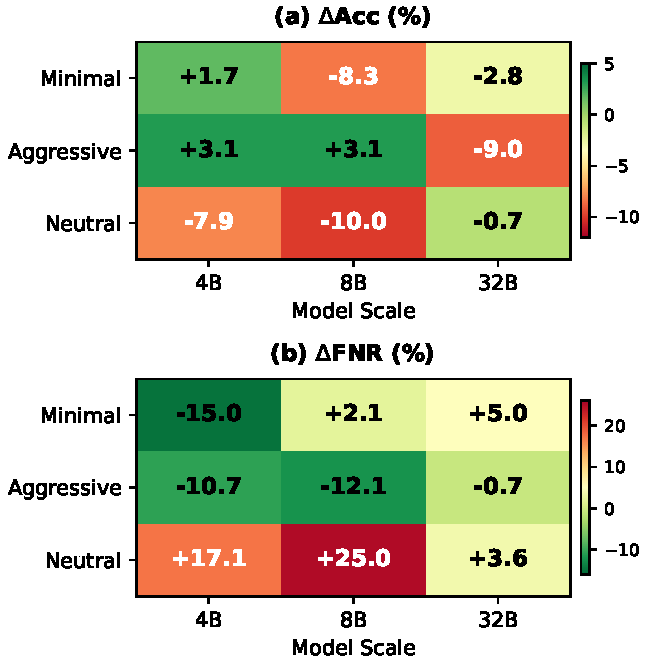
\includegraphics[width=\columnwidth]{fig_prompt_model_heatmap.pdf}
  \caption{Prompt-model interaction heatmap. (a) Accuracy delta ($\Delta$Acc) and (b) FNR delta ($\Delta$FNR) for each model-prompt combination. In the evaluated Qwen settings, 4B prefers Minimal, 8B prefers Aggressive, and Neutral is consistently weaker.}
  \label{fig:supp_heatmap}
\end{figure}

Figure~\ref{fig:supp_heatmap} visualizes the prompt-model interaction across all configurations. Key observations:

\begin{itemize}
  \item \textbf{4B models prefer Minimal prompts}: concise instructions yield the best accuracy and FNR improvements, suggesting that smaller models benefit from reduced instruction complexity.
  \item \textbf{8B models prefer Aggressive prompts}: detailed, category-aware instructions help mid-scale models leverage their stronger reasoning capabilities.
  \item \textbf{Neutral is weaker in the evaluated Qwen settings}: the middle-ground strategy fails to match either extreme, indicating that prompt design for ATR benefits from deliberate calibration rather than compromise.
\end{itemize}

%% ============================================================
%% Appendix D: Main Result Visualization
%% ============================================================
\subsection{Additional Visualization}
\label{sec:appendix_main_result}

Figure~\ref{fig:main_result_supp} provides a visual summary of the main results on UCF-Crime ($N$=290). Three key observations emerge: (1)~ATR consistently improves accuracy over Baseline for both 4B and 8B configurations, with both surpassing the 32B Baseline (dashed line); (2)~the primary source of ATR's gain is FNR reduction -- 4B+Minimal drops from 26.4\% to 11.4\%, recovering anomalies that Baseline misses due to attention dilution; (3)~Clip-Only suffers catastrophic FPR inflation (96.4\% for 4B), confirming that local evidence without global context leads to systematic over-prediction.

\begin{figure}[h]
  \centering
  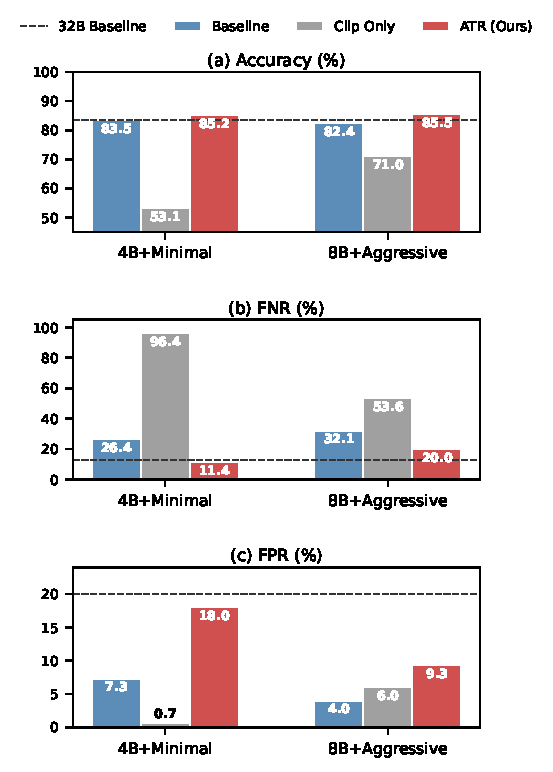
\includegraphics[width=\columnwidth]{fig_main_result.pdf}
  \caption{Main result comparison: Accuracy, FNR, and FPR for Baseline, Clip-Only, and ATR across two primary configurations (4B+Minimal, 8B+Aggressive) with 32B Baseline as reference (UCF-Crime, $N$=290).}
  \label{fig:main_result_supp}
\end{figure}

\bibliography{references}

% Complete and enable the official checklist before submission.
% \input{ReproducibilityChecklist.tex}

\end{document}
